\documentclass[../manuale_utente.tex]{subfiles}
\begin{document}


\subsection{Creazione workflow}
    \label{sub:crea_work}
\subsubsection{Caricamento dati}
    \label{subsub:carica_dati}

Il primo passo per poter utilizzare HD-Viz è importare dei dati. È possibile farlo in due modi:
\begin{itemize}
    \item caricamento di dati tramite file \glossario{CSV} da locale
    \item caricamento di dati tramite query da un database esterno
\end{itemize}
In seguito l’utente potrà esplorare e manipolare i grafici al fine di analizzare i dati, trarne conclusioni e similitudini tra essi. \\
Per importare un file da locale è sufficiente andare nella sezione \emph{“Carica file”}  in alto a sinistra, cliccare su \emph{“scegli file”}, 
scegliere un file CSV presente sul proprio dispositivo e poi cliccare su \emph{“Carica”}. 
Per importare dati tramite database bisogna cliccare sul bottone \emph{“Carica”} presente nel riquadro in alto a sinistra, relativo al caricamento database.
In questo modo il database verrà caricato tramite un file di configurazione presente nella cartella  \verb|server/src/dbConfig|

\begin{figure}[H]
	\centering
	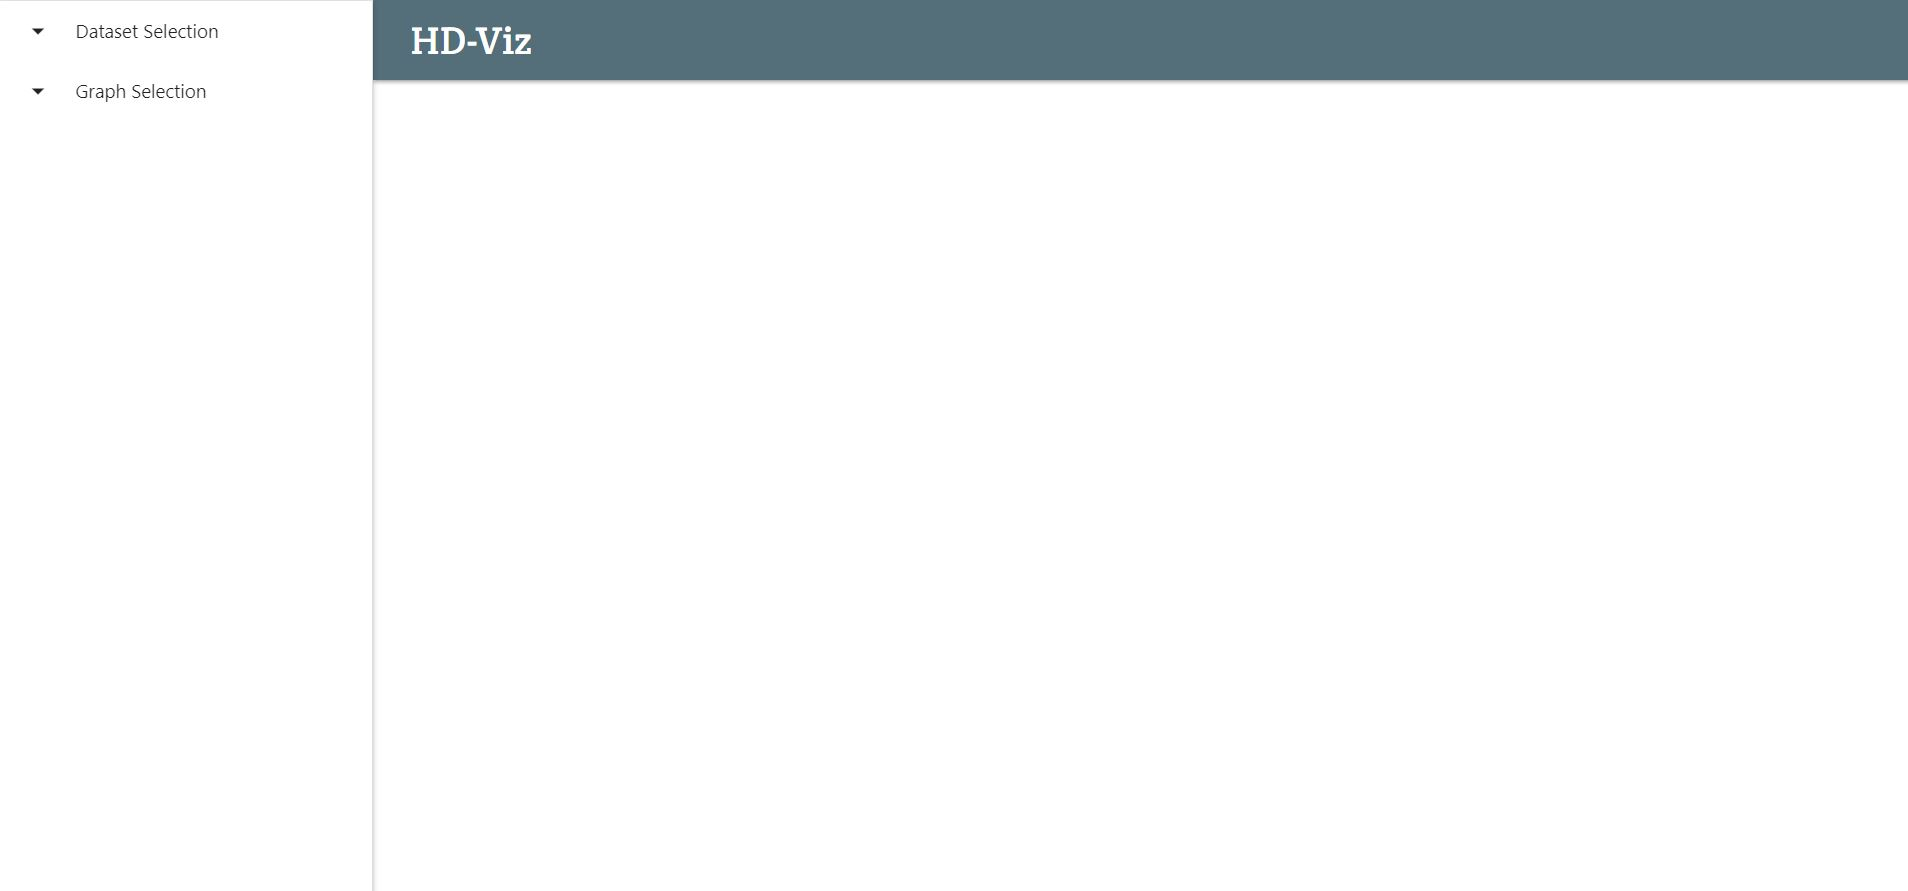
\includegraphics[width=18cm]{src/img/introduzione.jpg}
	\caption{Introduzione a Hd-Viz}
\end{figure}

%\begin{figure}[H]
%	\centering
%	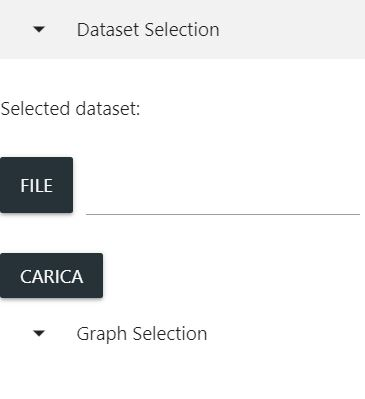
\includegraphics[width=18cm]{src/img/seleziona_dataset.jpg}
%	\caption{Seleziona fonte}
%\end{figure}


\subsubsection{Visualizzazione grafico}
    \label{subsub:vis_graf}
Una volta che il file è stato caricato, il grafico principale, lo \glossario{ScatterPlot Matrix}, verrà definito con i dati appena passati. \\
Grazie al menu a tendina in alto a sinistra sarà possibile cambiare grafico passando per esempio al Force Field, all’Heat Map e alla Distance Map.

\begin{figure}
	\centering
	\begin{minipage}{.5\textwidth}
	  \centering
	  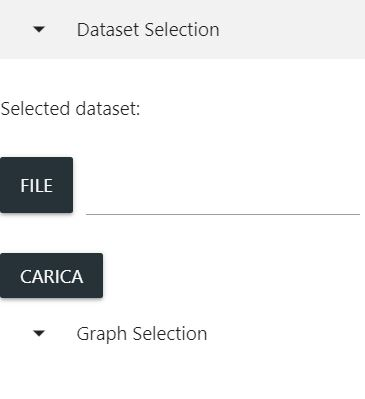
\includegraphics[width=.5\linewidth]{src/img/seleziona_dataset.jpg}
	  \caption{Seleziona fonte}
	  \label{fig:sub1}
	\end{minipage}%
	\begin{minipage}{.5\textwidth}
	  \centering
	  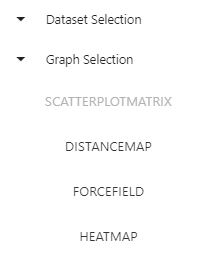
\includegraphics[width=.5\linewidth]{src/img/seleziona_grafico.jpg}
	  \caption{Seleziona grafico}
	  \label{fig:sub2}
	\end{minipage}
	\caption{Selezione fonte e grafico}
	\label{fig:test}
\end{figure}

\newpage

\paragraph{ScatterPlot Matrix}
    \label{par:vis_scatt}
Si tratta di un grafico che permette di visualizzare la relazione tra due variabili quantitative riportate su uno spazio cartesiano. Ogni unità statistica è rappresentata da un punto posizionato sul grafico in base alle sue coordinate. 
Quindi questo grafico sarà costituito da tanti punti quante sono le unità statistiche oggetto di studio. I valori che assume l’unità statistica per le due variabili rappresentano quindi la posizione dell’unità rispetto agli assi. 
Osservando l’andamento dei punti si può notare come sembra esserci una relazione lineare positiva o negativa. Se il modello di punti sul grafico scende dall'alto a sinistra verso il basso a destra, suggerisce una correlazione negativa. 
Può essere disegnata una linea di andamento (o linea di trend) per studiare la correlazione tra le variabili in esame. Se non c’è relazione tra le due variabili all’aumentare dei valori di una variabile, i valori dell’altra variabile non risulteranno in media né aumentare né diminuire.\\
In questo grafico sarà possibile modificare la dimensione del dataset, la dimensione della matrice, modificarne la dimensione rappresentata mediante tinta, mediante brillanza. Tutti questi parametri si troveranno
in ordine in un menu a sinistra. Ad ogni manipolazione dei parametri inseriti si otterrà subito una modifica del grafico. \\
Qui di seguito per esempio ecco come si mostra uno ScatterPlot Matrix al caricamento dei dati dell'Iris.

\begin{figure}[H]
	\centering
	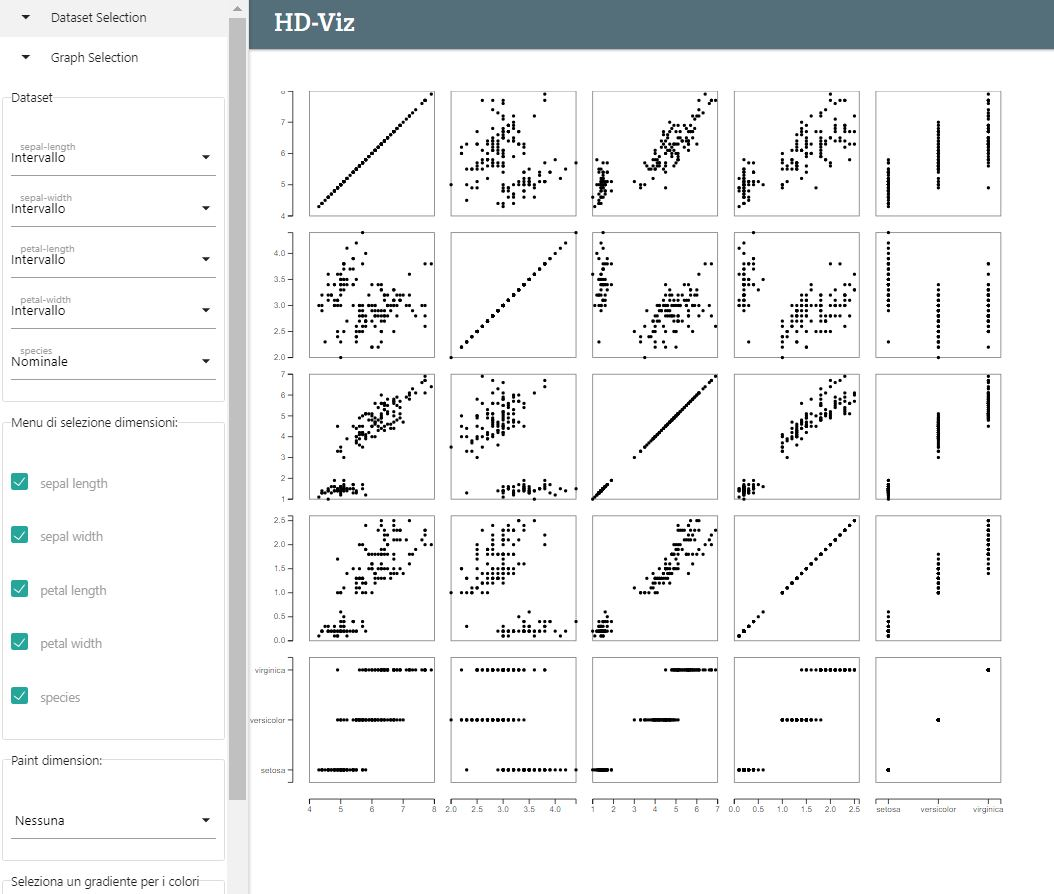
\includegraphics[width=18cm]{src/img/spm/spm_iris.jpg}
	\caption{ScatterPlot Matrix iris dataset}
\end{figure}

Quando si va a dare colore alla lunghezza dei sepali, il risultato è il seguente:

\begin{figure}[H]
	\centering
	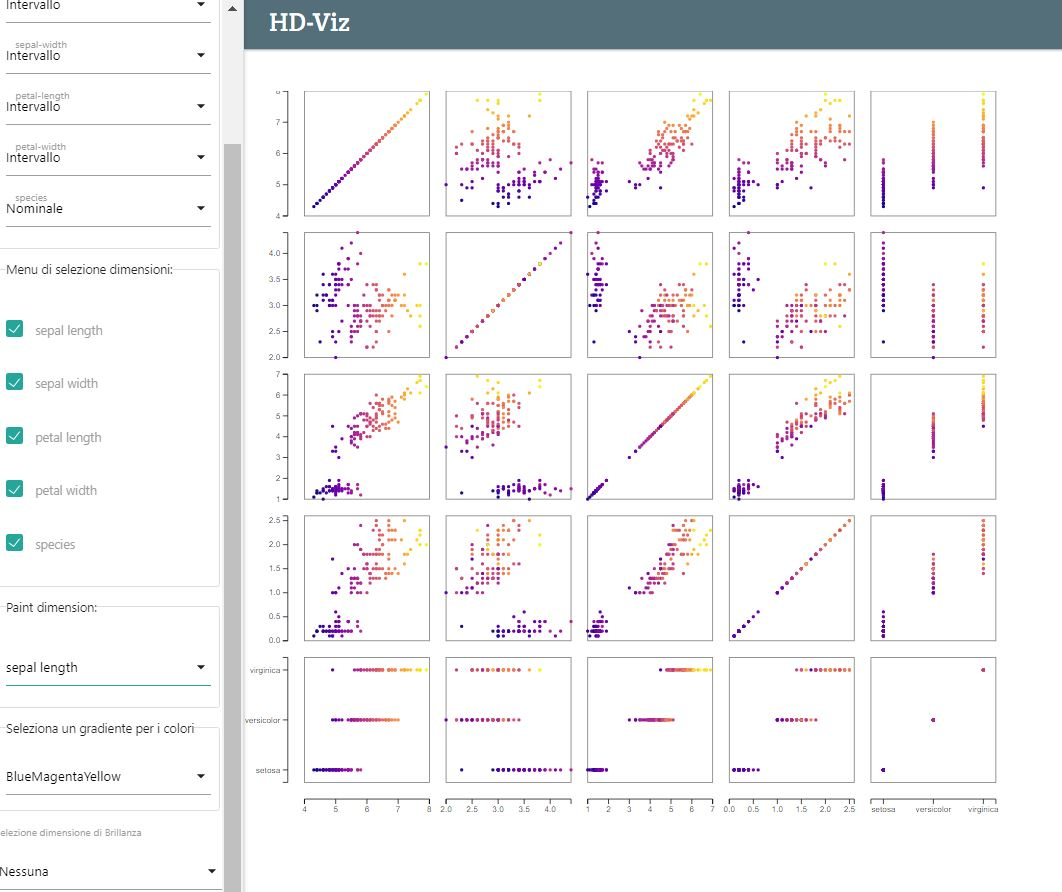
\includegraphics[width=18cm]{src/img/spm/spm_colore_dimensione_sepal.jpg}
	\caption{ScatterPlot Matrix lunghezza del sepalo colorato}
\end{figure}

È possibile inoltre cambiare i colori rappresentati. Nel seguente esempio si è scelto di colorare la dimensione del sepalo, e si è usato come gradiete il CoolWarm.

\begin{figure}[H]
	\centering
	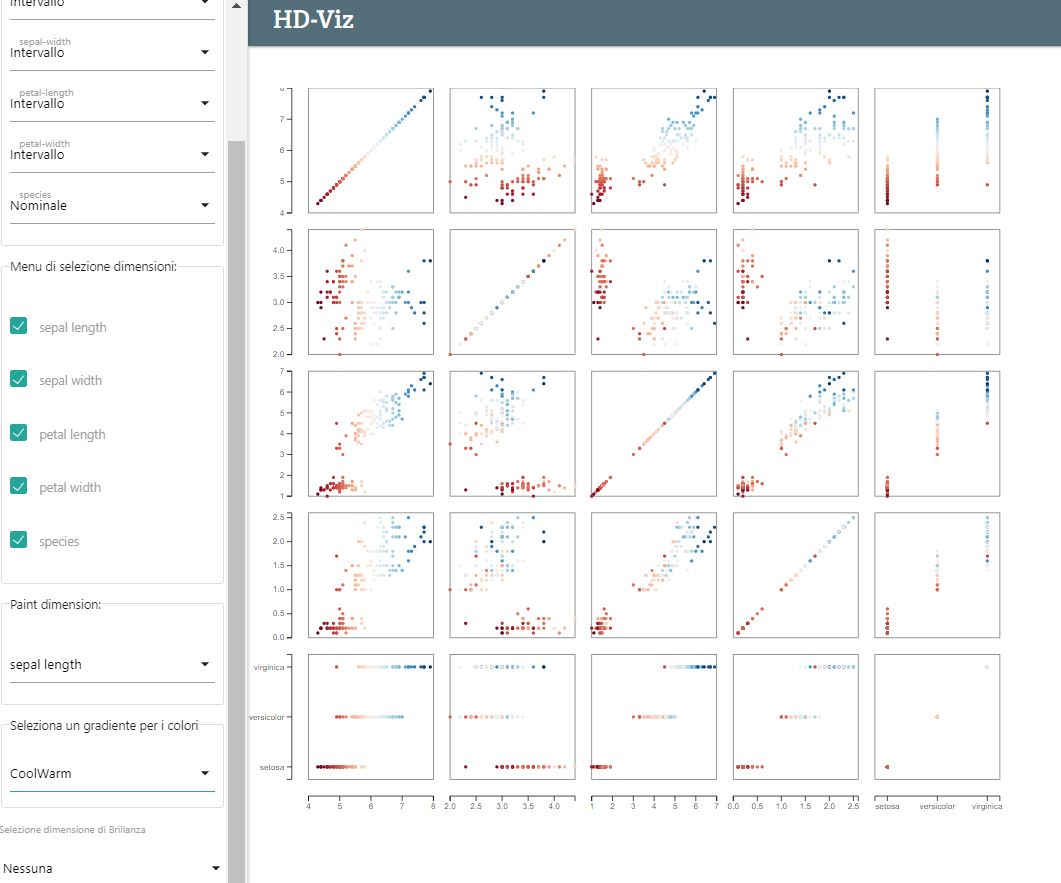
\includegraphics[width=18cm]{src/img/spm/spm_mix_colori.jpg}
	\caption{ScatterPlot Matrix modifica di più colori}
\end{figure}


È possibile cambiare le dimensioni rappresentate escludendone una ed aggiungendone un'altra, cliccando sulla checkbox associata alla dimensione che vogliamo escludere/aggiungere.

\begin{figure}[H]
	\centering
	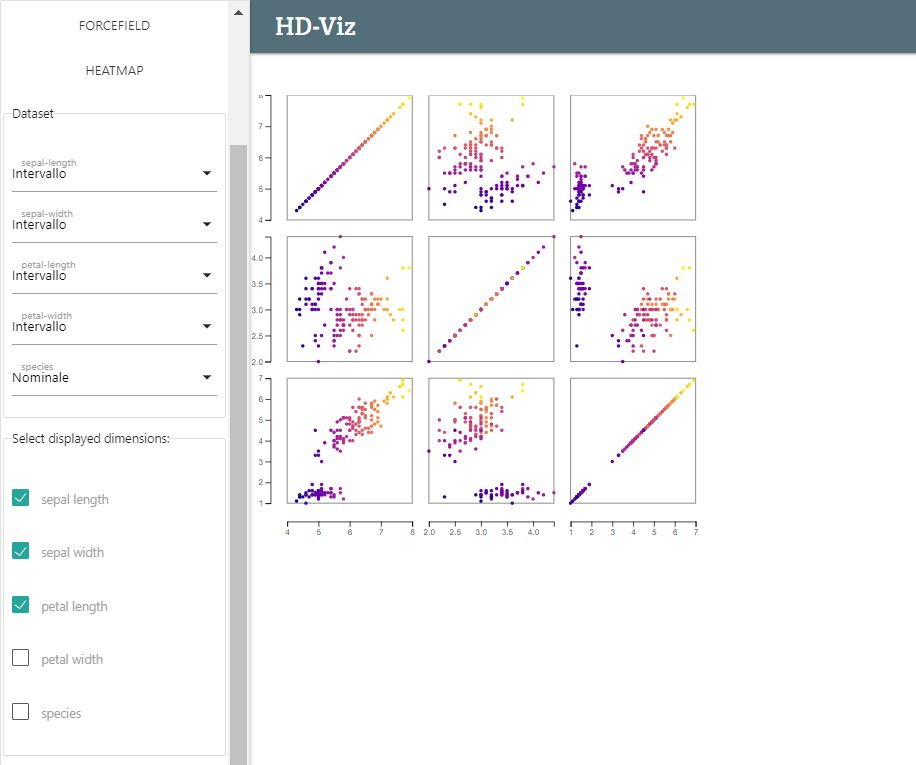
\includegraphics[width=18cm]{src/img/spm/spm_cambio_dim.jpg}
	\caption{ScatterPlot Matrix modifica delle dimensioni rappresentate}
\end{figure}


\paragraph{Distance Map}
    \label{par:vis_distance}
Si occupa di misurare la similarità di due unità statistiche adottando diversi algoritmi di calcolo.\\
Dopo aver selezionato la visualizzazione Distance Map in alto a sinistra, varie opzioni per la manipolazione delle distanze compaiono nel menu sottostante. Qui ad esempio si mostra come appare il dataset dell'Iris
dopo aver selezionato la visualizzazione Distance Map e modificato opportunamente i metadati di tipo:

\begin{figure}[H]
	\centering
	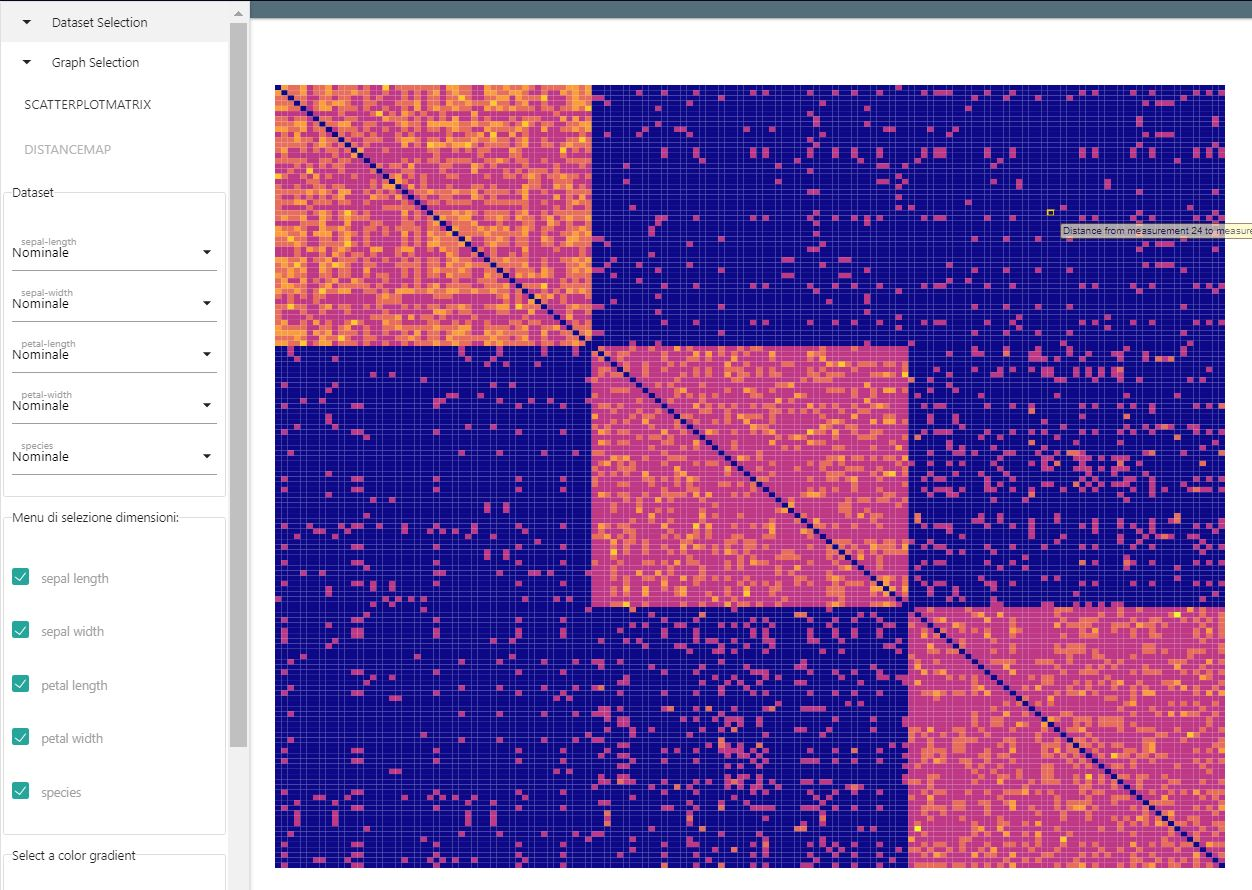
\includegraphics[width=18cm]{src/img/dm/iris_base_dm.jpg}
	\caption{Distance Map applicata all'Iris}
\end{figure}

Come per ScatterPlot, è possibile ridurre il dataset tramite le impostazioni presenti a sinistra.
Inoltre, è possibile manipolare impostazioni come l'algoritmo utilizzato per il calcolo della distanza, per l'assegnazione di pesi alle dimensioni, per standardizzare i dati e per clusterizzare unità statistiche tra loro vicine. Ogni manipolazione modifica dinamicamente la visualizzazione, permettendo all'analista di estrarre informazioni dai dati.\\
Di seguito per esempio si mostra come appare il dataset dell'Iris dopo aver selezionato come colore la scala di grigi, e l'ordinamento "Hierarichal Clustering".


\begin{figure}[H]
	\centering
	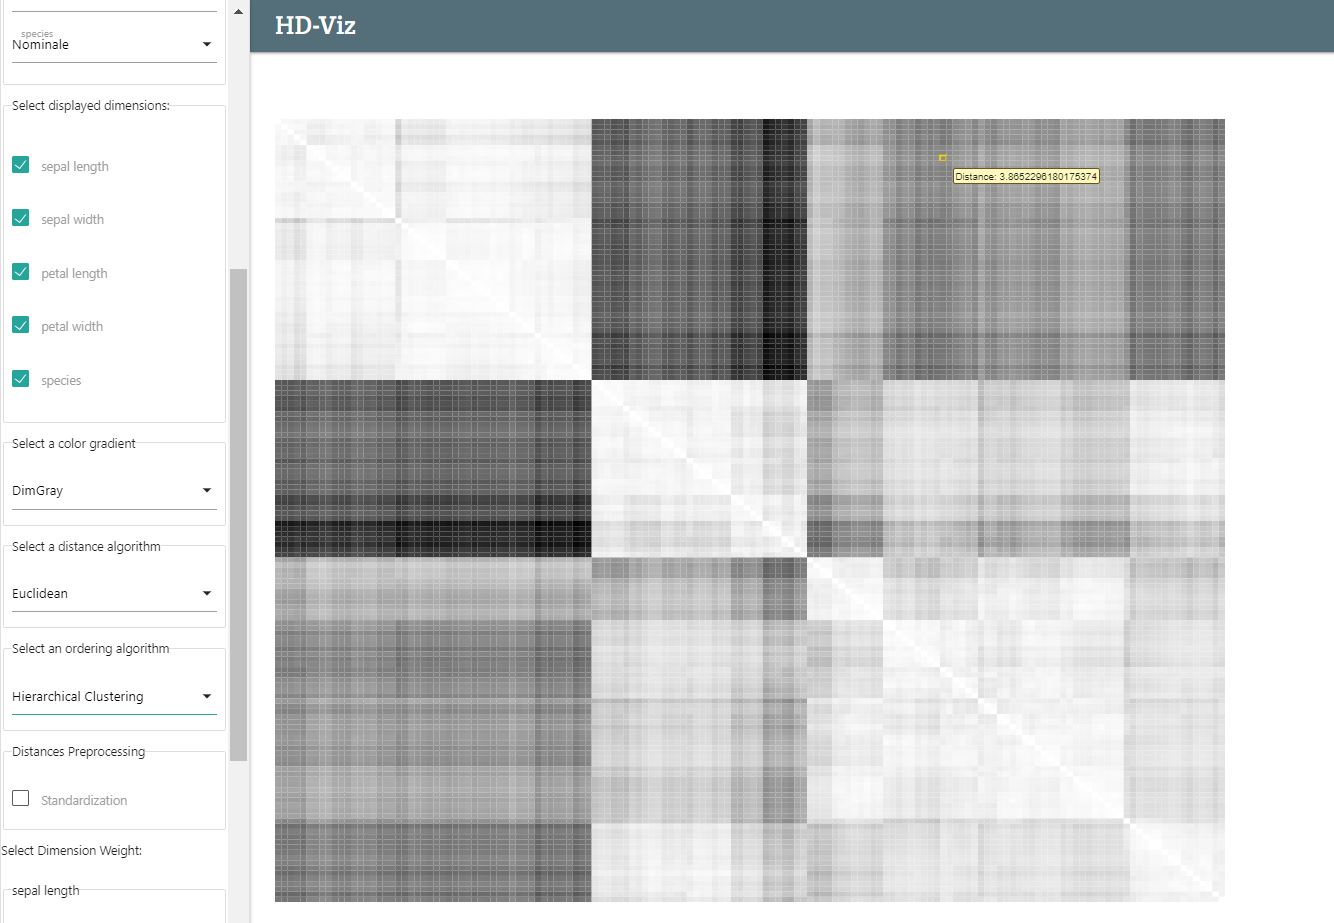
\includegraphics[width=18cm]{src/img/dm/iris_clustering_euclideo_dm.jpg}
	\caption{DistanceMap applicata all'Iris}
\end{figure}


\paragraph{Force Field}
    \label{par:vis_force_field}
Il grafico \glossario{Force Field} traduce le distanze tra unità statistiche in forze di attrazione e repulsione tra queste unità. Permette di rappresentare proiettate nello spazio le unità statistiche sotto forma di nodi e le distanze tra loro come archi. 
Questo grafico esegue una riduzione dimensionale preservando, o addirittura evidenziando, le strutture ed i cluster presenti nei dati.  Al caricamento del grafico i punti si dispongono nello spazio in base alle forze a cui sono soggetti. 

\begin{figure}[H]
	\centering
	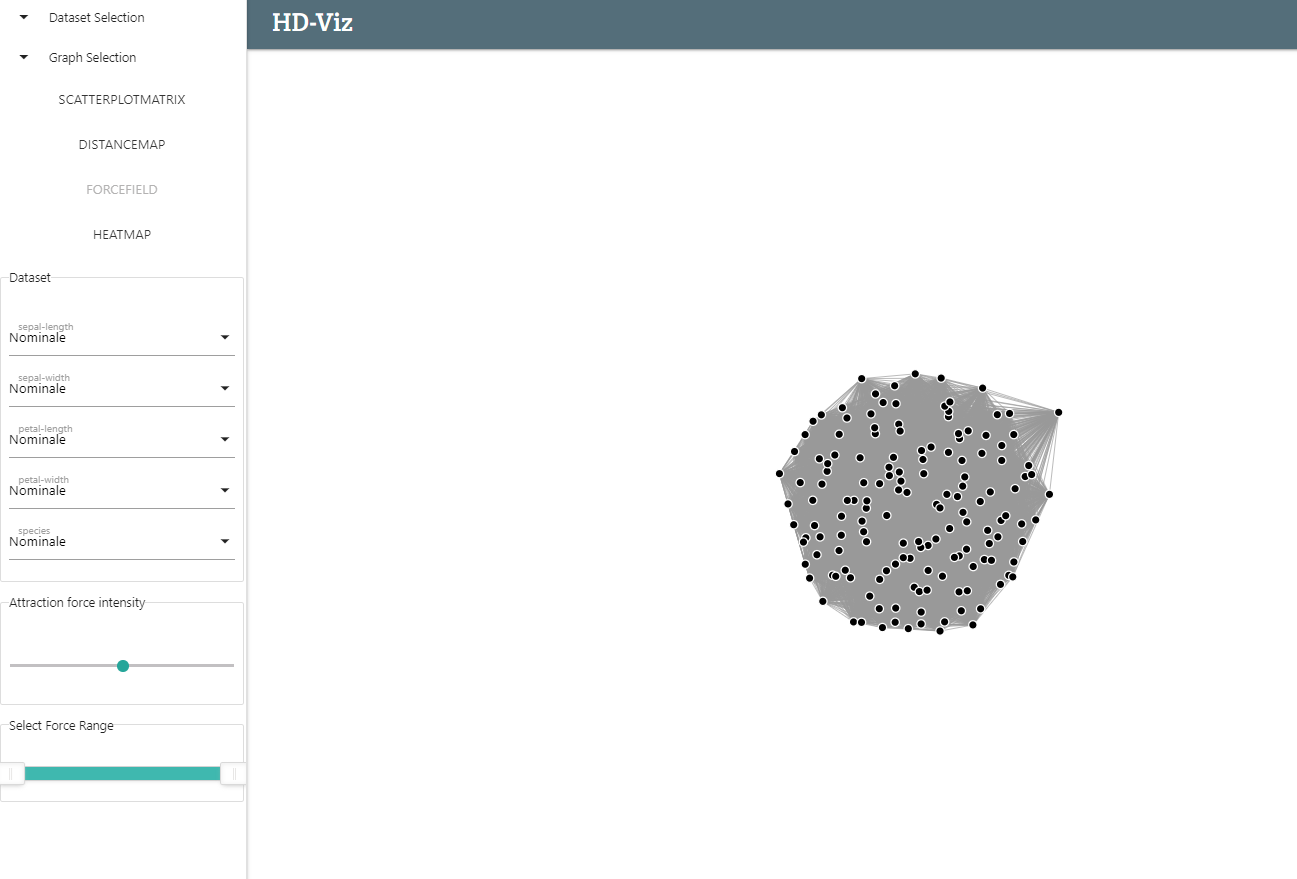
\includegraphics[width=18cm]{src/img/ff/ff_iris_0_1}
	\caption{ForceField applicata all'Iris - caricamento}
\end{figure}

Dopo poco si raggiunge una condizione di equilibrio. 

\begin{figure}[H]
	\centering
	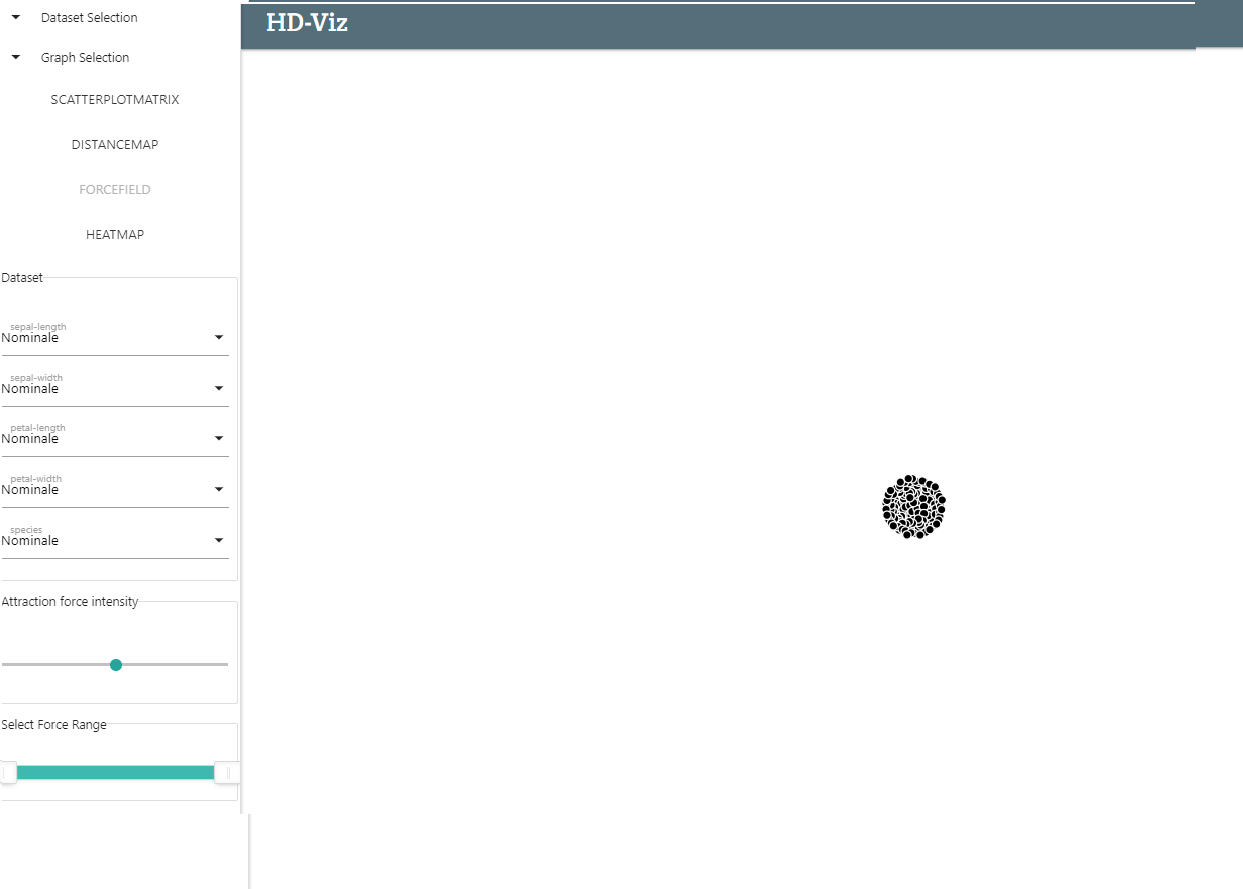
\includegraphics[width=18cm]{src/img/ff/ff_iris_0_2}
	\caption{ForceField applicata all'Iris - equilibrio}
\end{figure}


Come per gli altri grafici è possibile manipolare il dataset ottenendo risultati differenti. Per esempio si può scalare la forza di attrazione tra nodi e si possono tagliare gli archi che collegano nodi con distanze al di fuori di quelle specificate

\begin{figure}[H]
	\centering
	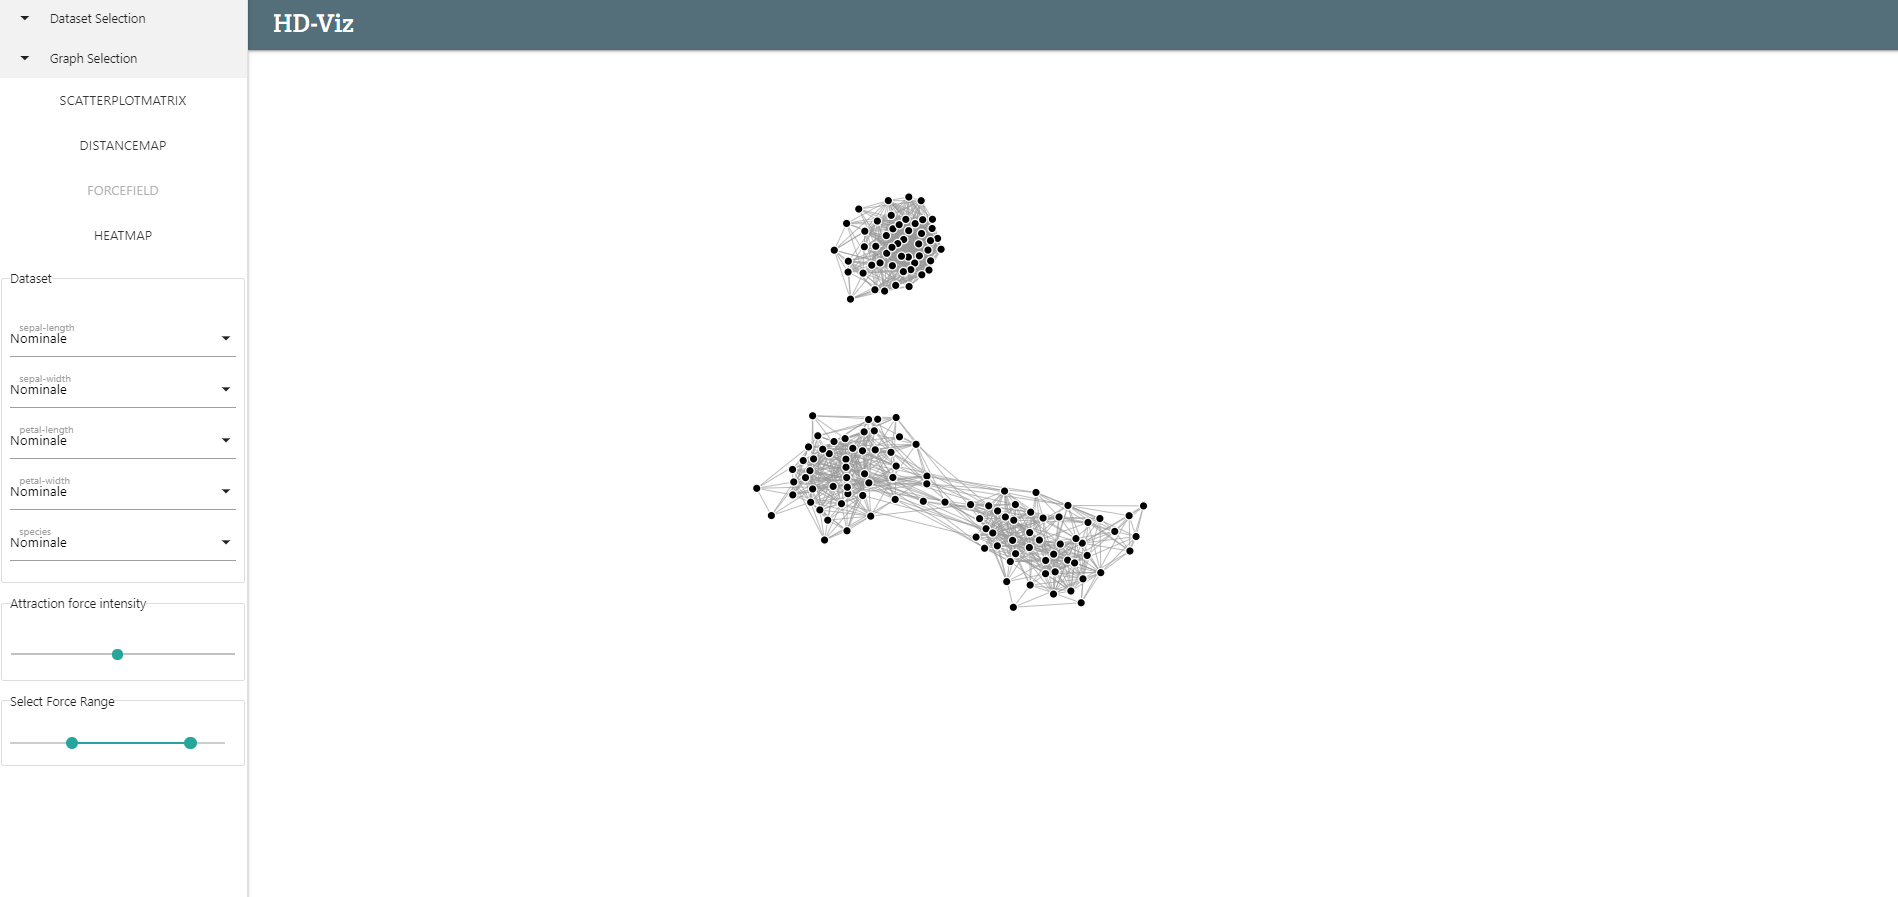
\includegraphics[width=18cm]{src/img/ff/ff_iris_1}
	\caption{ForceField applicata all'Iris - modifica dataset}
\end{figure}


Il ForceField è caratterizzato dalla possibilità di modificare le forze di attrazione, e il rispettivo range. Ad ogni manipolazione si possono ottenere quindi risultati differenti, 
come rappresentato di seguito:

\begin{figure}[H]
	\centering
	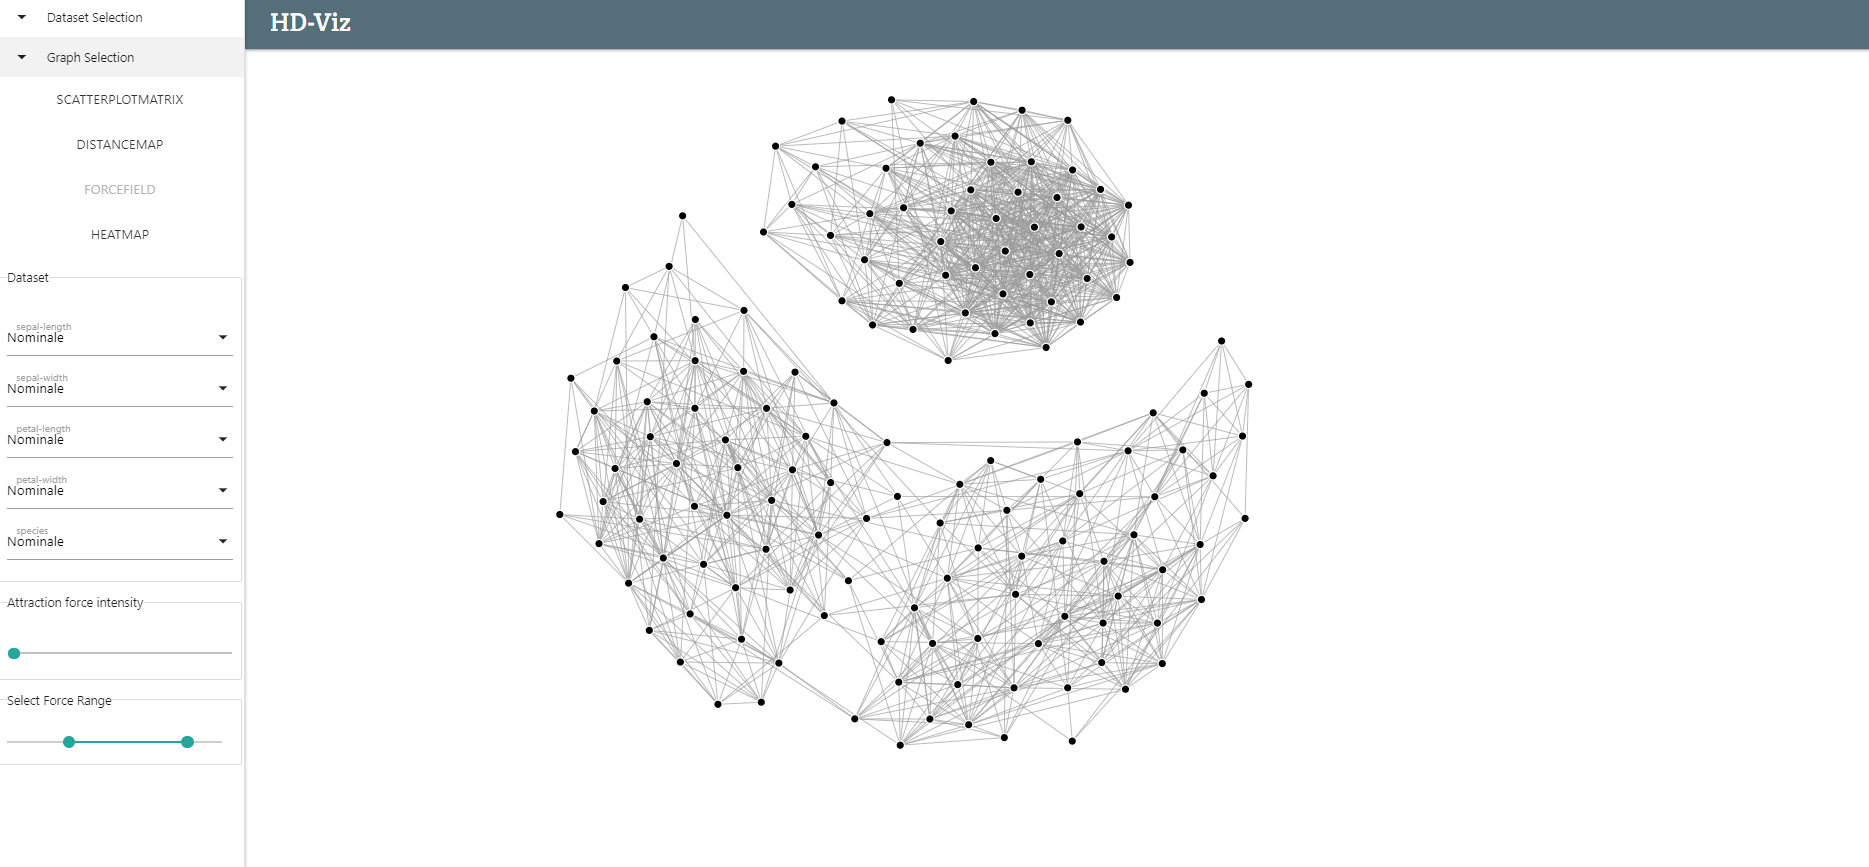
\includegraphics[width=18cm]{src/img/ff/ff_iris_2}
	\caption{ForceField applicata all'Iris - modifica force intensity}
\end{figure}

\begin{figure}[H]
	\centering
	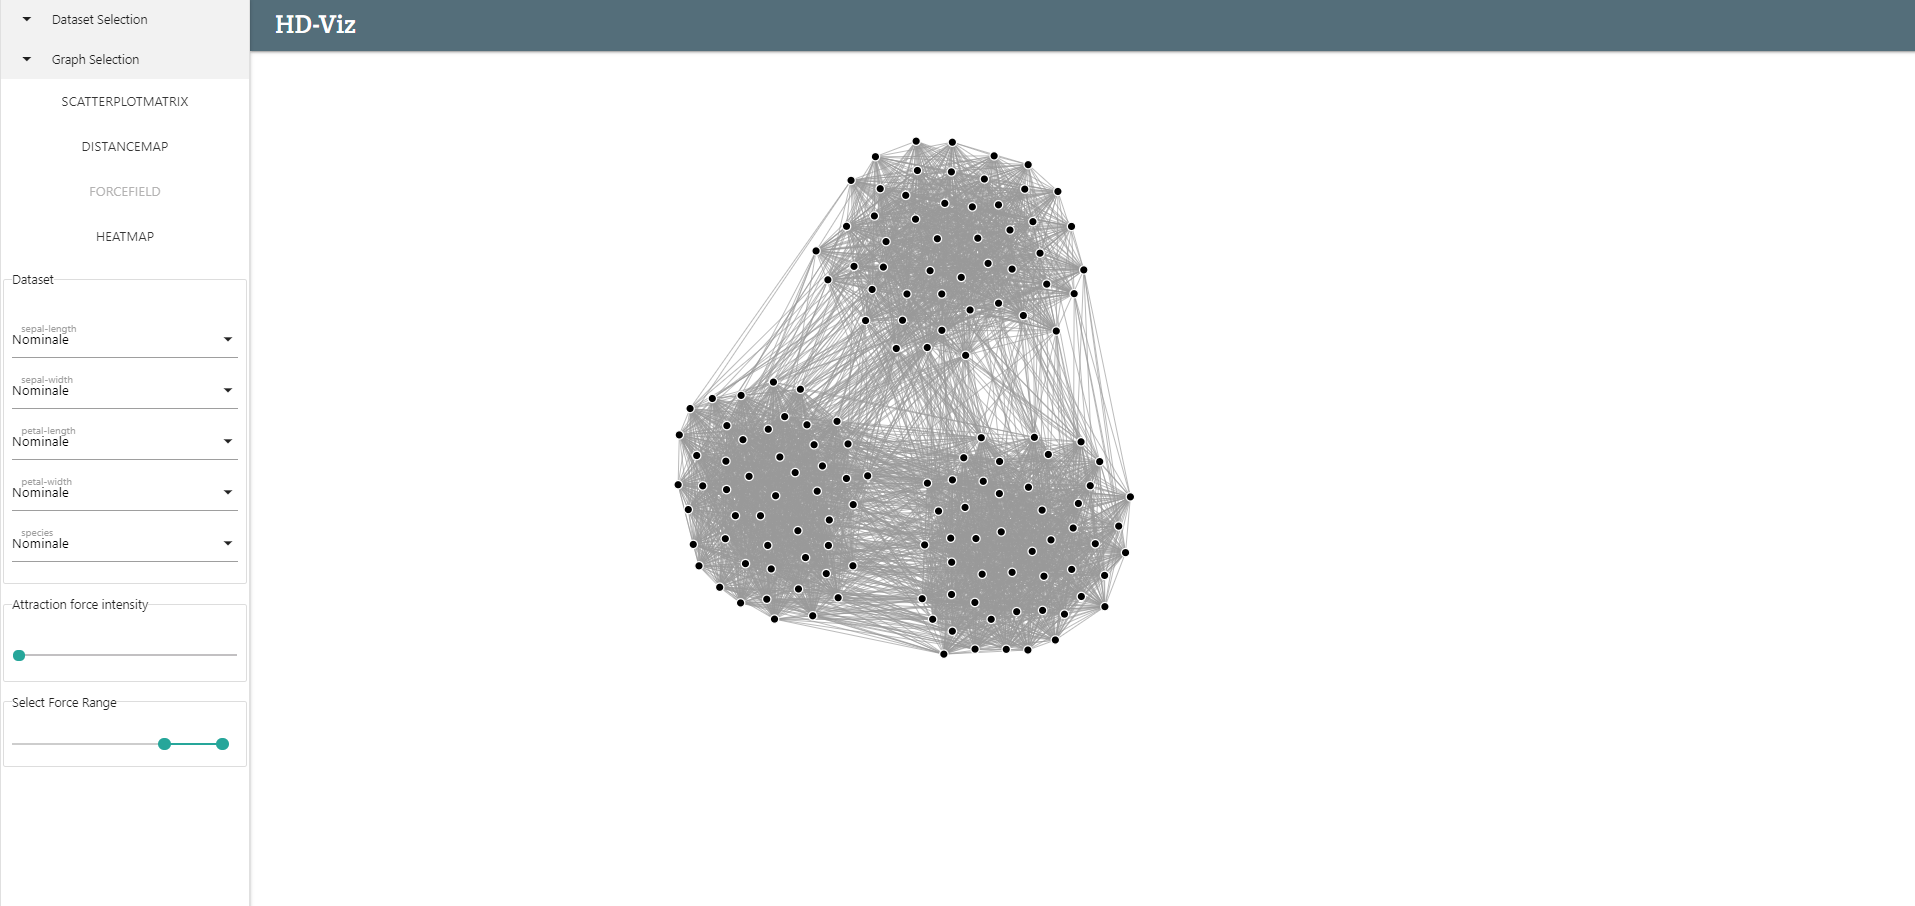
\includegraphics[width=18cm]{src/img/ff/ff_iris_3}
	\caption{ForceField applicata all'Iris - modifica force range}
\end{figure}

\begin{figure}[H]
	\centering
	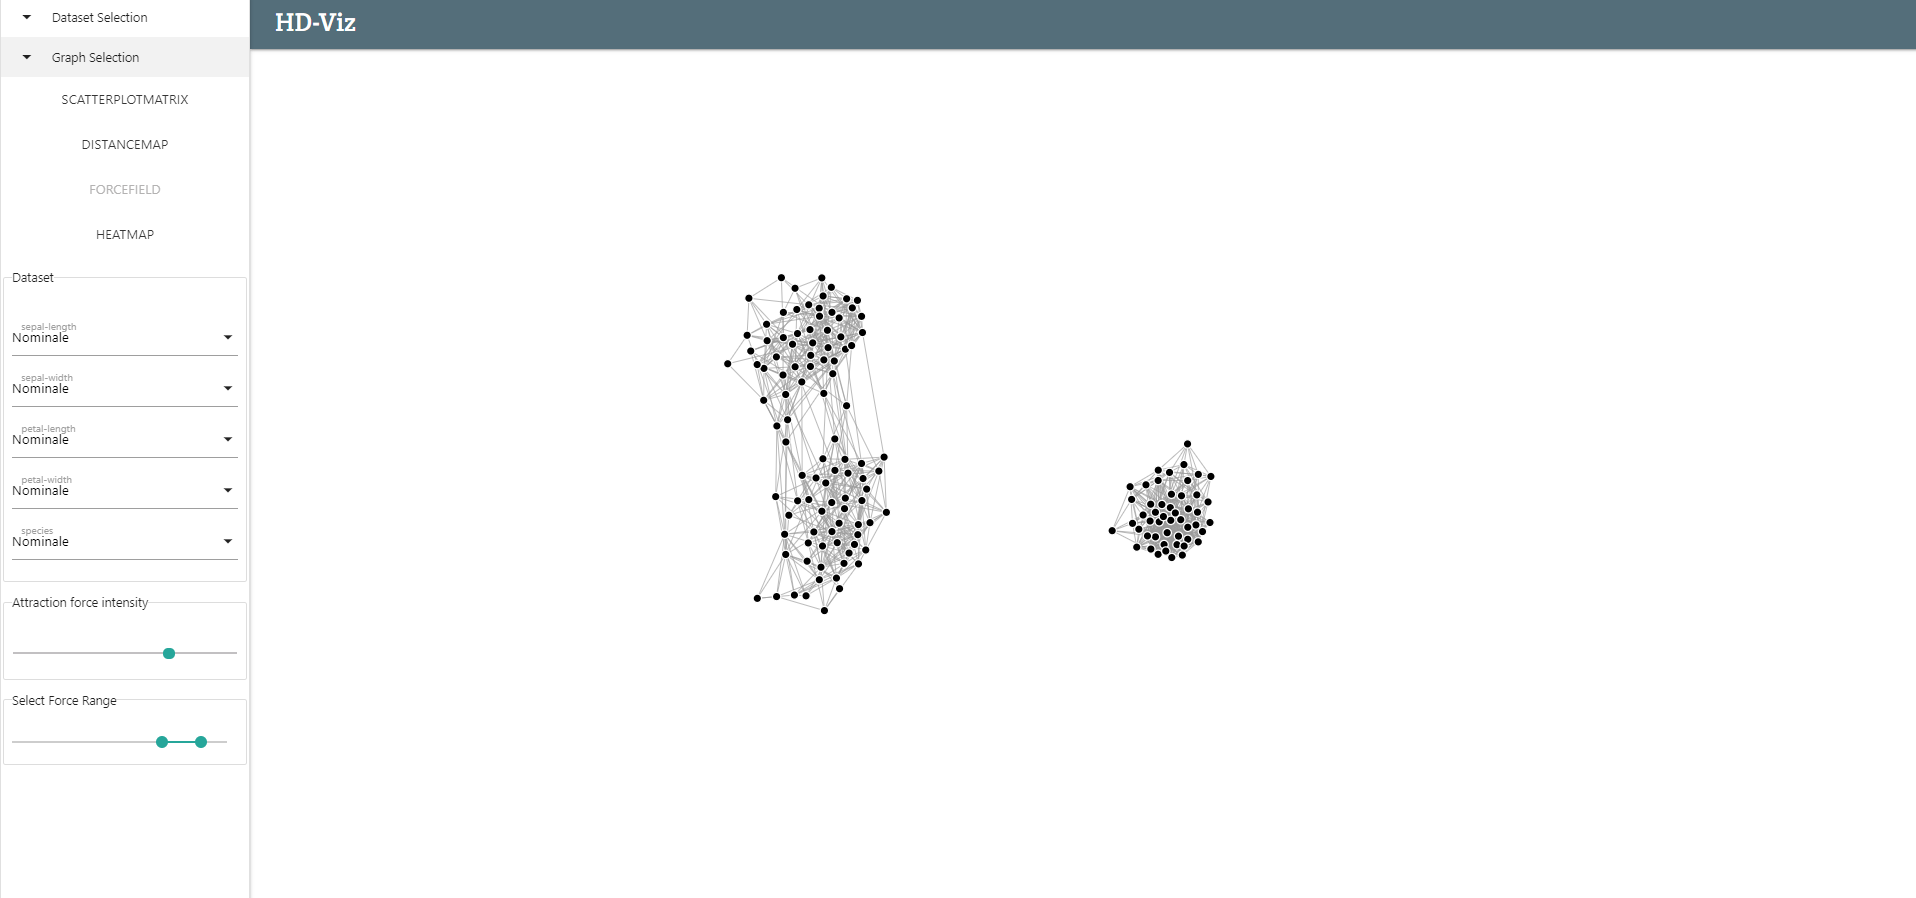
\includegraphics[width=18cm]{src/img/ff/ff_iris_4}
	\caption{ForceField applicata all'Iris - modifica force range e force intensity}
\end{figure}

È anche possibile interagire con i nodi e ridisporre dinamicamente i punti:

\begin{figure}[H]
	\centering
	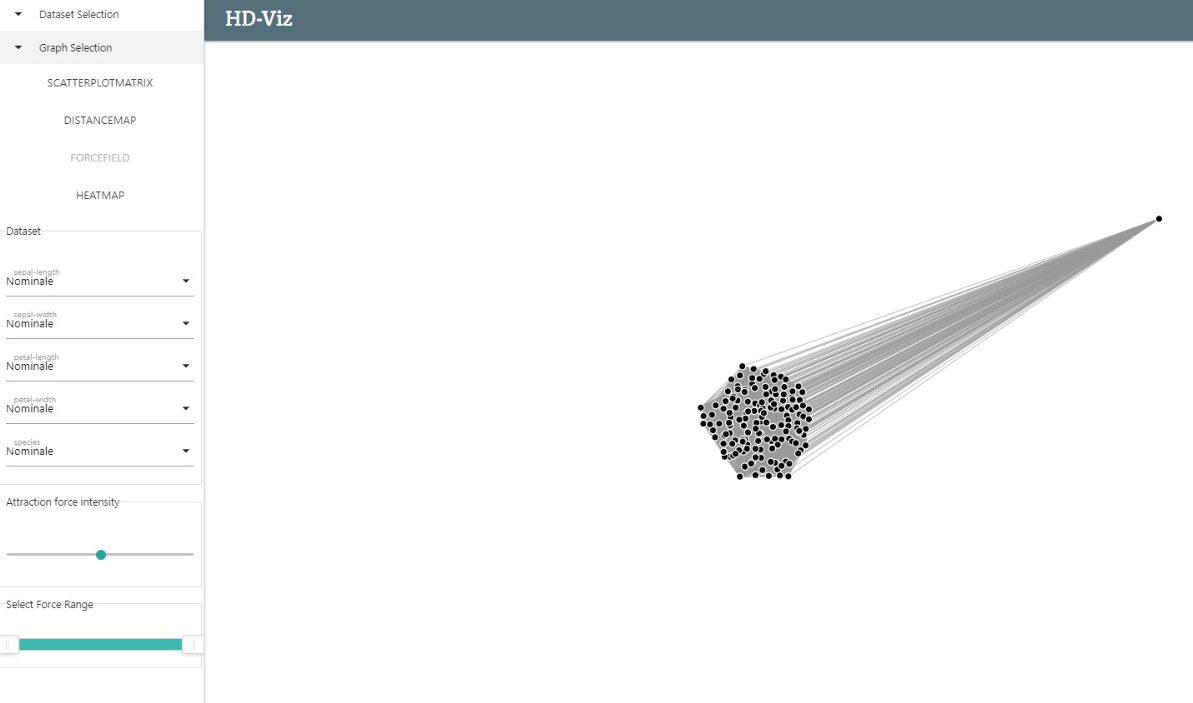
\includegraphics[width=18cm]{src/img/ff/ff_iris_5}
	\caption{ForceField applicata all'Iris - manipolazione dei punti}
\end{figure}

\paragraph{HeatMap}
    \label{par:vis_heatmap}

Il grafico \glossario{Heat map} trasforma i diversi valori delle dimensioni del dataset in colori più o meno intensi, permettendo di evidenziare eventuali ripetizioni o pattern all'interno del dataset. \\
Come per gli altri grafici è possibile usufruire delle impostazioni nel menu a sinistra per poter modificare il grafico. Qui di seguito si mostra la differenza tra scale cromatiche differenti:

\begin{figure}[H]
	\centering
	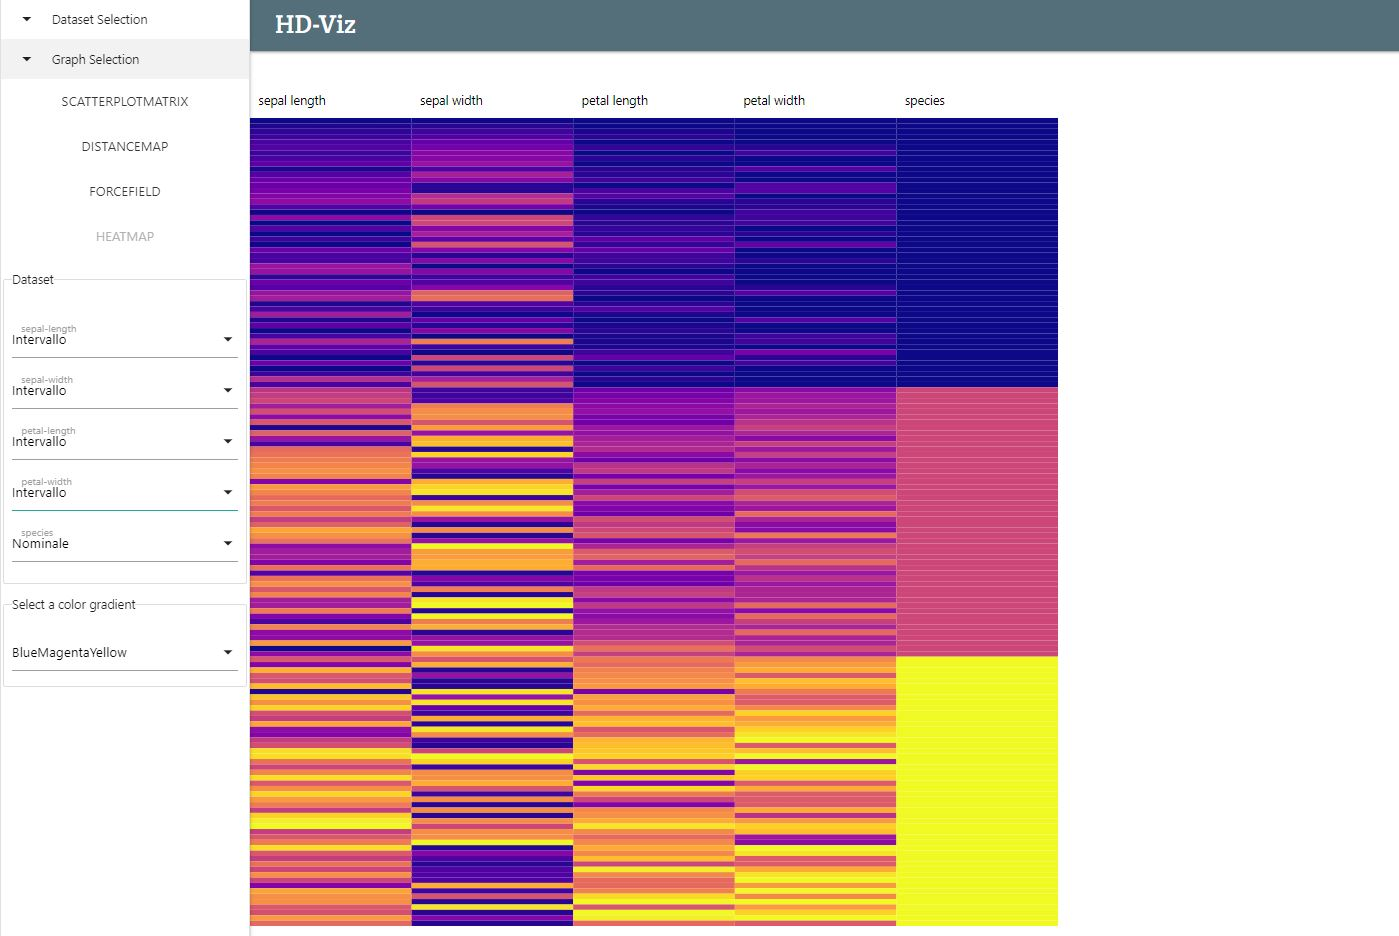
\includegraphics[width=18cm]{src/img/hm/heat_map_base.jpg}
	\caption{Heat Map base}
\end{figure}

\begin{figure}[H]
	\centering
	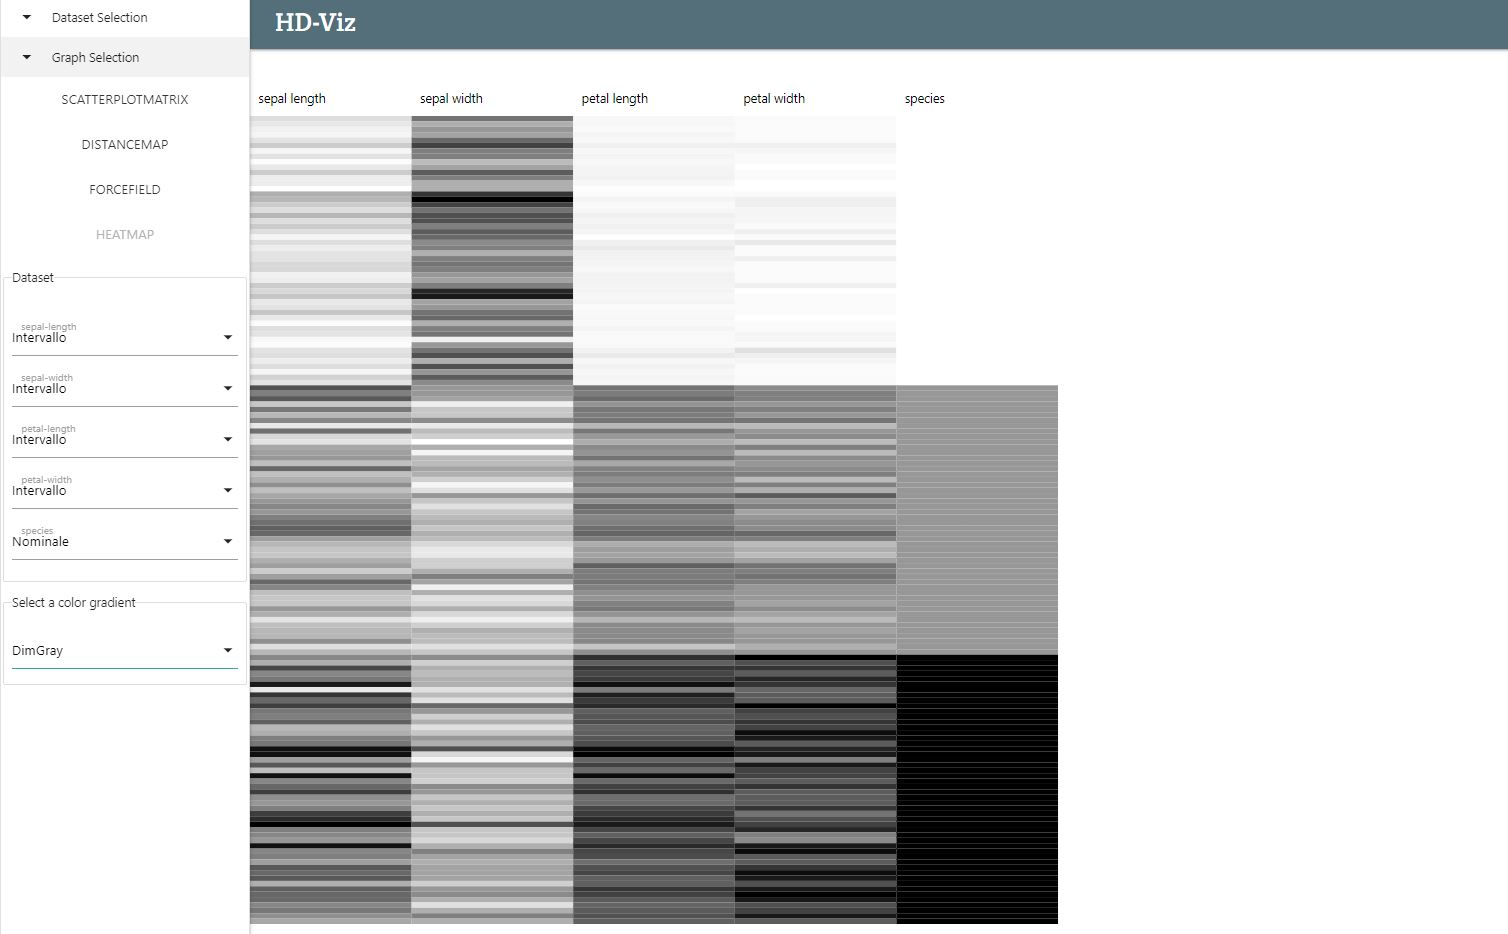
\includegraphics[width=18cm]{src/img/hm/heat_map_base_gray.jpg}
	\caption{Heat Map in scala di grigi}
\end{figure}




\end{document}